%%!TEX root=../main.tex

\section{Introduction}
\subsection{Tennis Games}
Tennis games are played on a rectangular court. According to the standard, the size of the court is 23.77 meters long. Since the tennis games could be separated into singles and doubles games. For the singles game, the wide is 8.2 meters and the doubles game is 11 meters. For each half of court, there are baseline, singles sidelines, doubles sidelines, server line and center service line. As shown in the figure \ref{Tennis court}, the distances are marked on the figure.

\begin{figure}[ht]
\centering
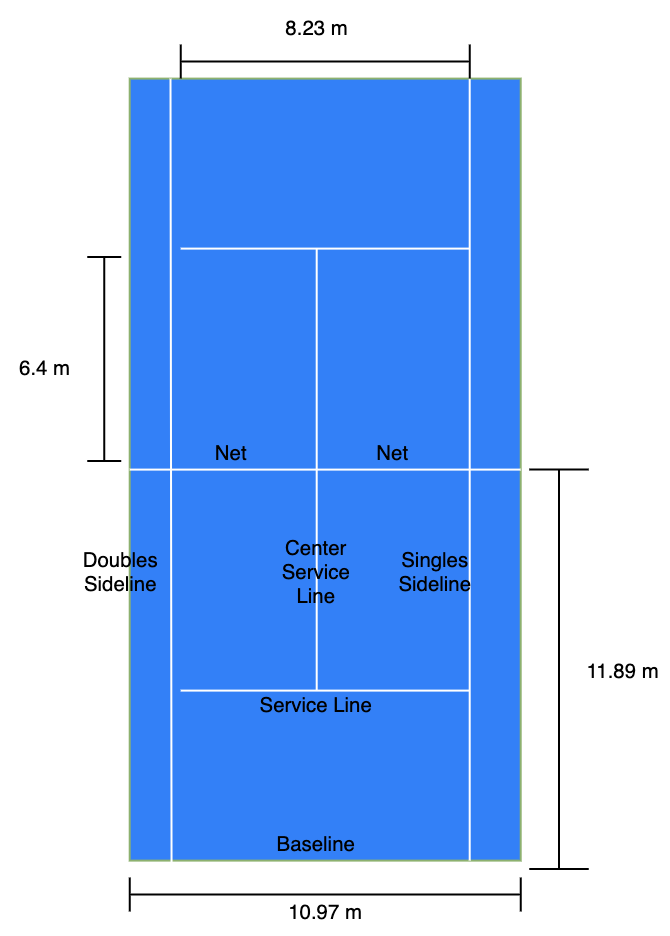
\includegraphics[width=2.5in]{\FIGDIR/P1_TennisCourt.png}
\caption{The Schematic Diagram of the Tennis Court}
\label{Tennis court}
\end{figure}

The players start on opposite sides of the court\cite{wiki:xxx}. Based on the result of tossing the coin, one side of players in the server and another is the receiver. The server could start from the areas surrounded by the baseline, the center service line and the sideline. The legal server should across the net and should not touch the net, diagonally drop into the service box of opponents. The receiver should hit back the ball before the ball dropping twice. The ball must cross the net and drop into the side of the opponent’s court.\\

\subsection{Predict localization of tennis ball}
The tennis courts have three categories: grass, clay and hard courts. The clay is the easiest material to judge since the drop point could leave a mark on the surface. But the grass and hard courts are relatively much harder to judge because of the high speed and the low bounce of the balls. Human eyes are not precise enough to capture the drop point of the ball and sometime could make it wrong. When the judgements are different between players and referees, the players are allowed to challenge point-ending line calls. Then the hawk-eye technology would be used on decision making.

The hawk-eye technology\cite{baodong2014hawkeye} \cite{gangal2007hawkeye} is the system consists of cameras and computers which could visually track the trajectory of the ball and display a record of its statistically most likely path as a moving image.  The principle\cite{chao2016tennis} is base on the triangulation that using visual images and timing data provided by the set cameras. Triangulation is the process of finding the location of a point by measuring the angles between the point and other points which are fixed.

Normally, more than 10 cameras \cite{lai2007study} which have about 120 MHz frame rate are set around the tennis court to capture the localization of the tennis, as shown in the figure \ref{Hawk-eye}. The signals and data are further sent to the high-speed video processor and update 100 times every second. The video processor would identify each frame from each camera, then transfers information to the computer for it to be turned into a 3D image and for the information to be collected into images such as a grouping corresponding pixels to the image of the ball. Then the computer would predict a ball path from the said 3D ball position as computed in successive frames and map the predicted path on the modeled area so as to identify any interaction with ball and lines.

\begin{figure}[ht]
\centering
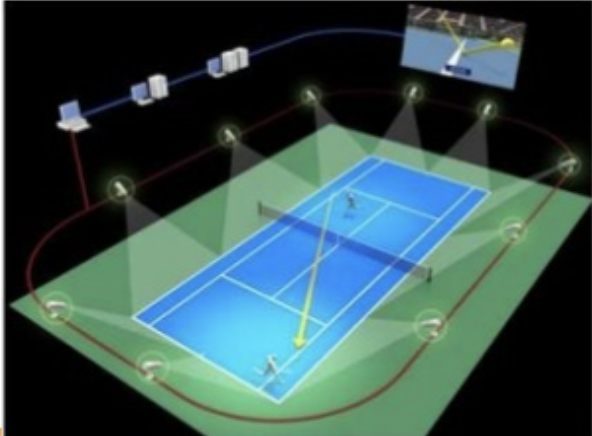
\includegraphics[width=3in]{\FIGDIR/P2_Hawkeye.png}
\caption{The Schematic Diagram of the Hawk-eye Technology}
\label{Hawk-eye}
\end{figure}

One of the advantages of hawk-eye technology is the system optimized human error in decision making. The collected data could further help the players to study from past games and improve their skills. However, there are several disadvantages that could not be avoided. Firstly, the lens distortion, the point spread caused by the scattering of the light and the distortion of pixels in digital photos could affect precision. Secondly, since the system should rapidly process the video feeds from the cameras. The quality of the video processor should be extremely high and would cause a high cost. Just imagine that if we would like to set the system in every match and every court.

With the development of sensor technology, the size of the sensor is becoming smaller and smaller. It's easier to set up sensors anywhere you need them. In addition, the cost of sensors is lower than that of professional motion cameras. So,a very tiny sensort could be set up on the tennis balls which could send a signal when the tennis ball drop on the ground which we could consider the tennis ball as a unknown node and then we can use various algorithm to predict the location of its drop point.In term of localization algorithms,they are becoming more and more mature and easy to understand and apply. People can choose different algorithms according to different scenes. Using the data obtained by sensors and machine learning technology, we can process and analyze the data to help the referee judge the game and improve the athletes' sports skills.\\
